\documentclass[tikz]{standalone}

\usetikzlibrary{matrix, positioning, automata, arrows}

\begin{document}

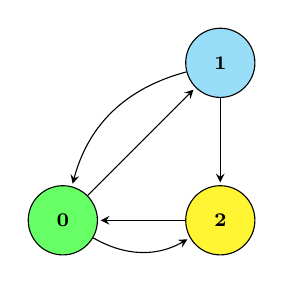
\begin{tikzpicture}[>=stealth, shorten >=1pt,node distance=2cm,on grid,auto, initial text = {}]
    \tikzstyle{every state}=[fill={rgb:black,1;white,10}]

    \node[state, fill=cyan!40]   (q_1) {\scriptsize $\textbf{1}$};
    \node[state, fill=yellow!80]   (q_3) [below of =q_1] {\scriptsize $\textbf{2}$};
    \node[state, fill=green!60]   (q_4) [left of =q_3] {\scriptsize $\textbf{0}$};


    \path[->]
    (q_1) edge  [bend right, above] (q_4)
    (q_4) edge   (q_1)
    (q_1) edge   (q_3)
    (q_3) edge   (q_4)
    (q_4) edge  [bend right, above] (q_3);
\end{tikzpicture}

\end{document}